\section{Band-Limited Convolution}
Let $x$ be an input tensor (e.g., a signal) and $y$ be another tensor representing the filter.
We denote the convolution operation as $x * y$.
Both $x$ and $y$ can be thought of as discrete functions (mapping tensor index positions $\mathbf{n}$ to values $x[\mathbf{n}]$). Accordingly, they have a corresponding Fourier  representation, which re-indexes each tensor in the spectral (or frequency) domain:
\[
F_x[\omega] = F(x[\mathbf{n}]) ~~~~~~~  F_y[\omega] = F(y[\mathbf{n}])
\] 
This mapping is invertible $x = F^{-1}(F(x))$. Convolutions in the spectral domain correspond to element-wise multiplications:
\[
x * y = F^{-1}(F_x[\omega] \cdot F_y[\omega])
\]
The intermediate quantity $S[\omega] = F_x[\omega] \cdot F_y[\omega]$ is called the \emph{spectrum} of the convolution. We start with the modeling assumption that for a substantial portion of the high-frequency domain, $|S[\omega]|$ is close to 0.
This assumption is substantiated by the recent work by Rahman et al. studying the inductive biases of CNNs~\cite{rahaman2018spectral}, with experimental results suggesting that CNNs are biased towards learning low-frequency filters (i.e., smooth functions). We take this a step further and consider the joint spectra of both the filter and the signal to understand the memory and computation implications of this insight.

\subsection{Compression}
Let $M_c[\omega]$ be a discrete indicator function defined as follows:
\[
M_c[\omega] = \begin{cases}
1, \omega \le c\\
0,\omega > c
\end{cases}
\]
$M_c[\omega]$ is a mask that limits the $S[\omega]$ to a certain \emph{band} of frequencies.
The \emph{band-limited} spectrum is defined as, $S[\omega] \cdot M_c[\omega]$,
and the band-limited convolution operation is defined as:
\begin{align*}
 x *_c y & = F^{-1}\{(F_x[\omega] \cdot M_c[\omega]) \cdot (F_y[\omega] \cdot M_c[\omega])\} \tag{1}\\
 & = F^{-1}(S[\omega] \cdot M_c[\omega]) \tag{2}  
\end{align*}
The operation $*_c$ is compatible with automatic differentiation as implemented in popular deep learning frameworks such as \textsf{PyTorch} and \textsf{TensorFlow}. The mask $M_c[\omega]$ is applied to both the signal $F_x[\omega]$ and filter $F_y[\omega]$ (in equation 1) to indicate the compression of both arguments and fewer number of element-wise multiplications in the frequency domain.

\subsection{FFT Implementation}
We implement band-limited convolution with the Fast Fourier Transform. % (a direct application of the equations above). 
FFT-based convolution is supported by many Deep Learning libraries (e.g., cuDNN).
It is most effective for larger filter-sizes where it significantly reduces the amount of floating point operations. While convolutions can be implemented by many algorithms, including matrix multiplication  and the Winograd minimal filtering algorithm, the use of an FFT is actually important (as explained above in section~\ref{whyFFTConvolution}).
The compression mask $M_c[\omega]$ is sparse in the Fourier domain.
$F^{-1}(M_c)$ is, however, dense in the spatial or temporal domains. %(corresponds to a $\text{sinc}()$ function). %SK: note this is not a typo sinc(x) = sin(x)/(x)
If the algorithm does not operate in the Fourier domain, it cannot take advantage of the sparsity in the frequency domain.

\subsubsection{The Expense of FFT-based Convolution}
It is worth noting that pre-processing steps are crucial for a correct implementation of convolution via FFT. The filter is usually much smaller (than the input) and has to be padded with zeros to the final length of the input signal. The input signal has to be padded on one end with as many zeros as the size of the filter to prevent the effects of wrapped-around filter data (for example, the last values of convolution should be calculated only from the final overlap of the filter with the input signal and should not be polluted with values from the beginning of the input signal). 

Due to this padding and expansion, FFT-based convolution implementations are often expensive in terms of memory usage.  Such an approach is typically avoided on GPU architecture, but recent results suggest improvements on CPU architecture~\cite{aleks2018fft}. 
The compression mask $M_c[\omega]$ reduces the size of the expanded spectra; we need not compute the product for those values that are masked out. Therefore, 
a band-limiting approach has the potential to make FFT-based convolution more practical for smaller filter sizes.

\subsubsection{Band-limiting technique}
We present the transformations from a natural image to a band-limited FFT map in Figure~\ref{fig:transforms}.

The FFT domain cannot be arbitrarily manipulated as we must preserve \emph{conjugate symmetry}.
For a  1D signal this is straight-forward. $F[-\omega] = F^{*}[\omega]$, where the sign of the imaginary part is opposite when $\omega<0$. The compression is applied by discarding the high frequencies in the first half %(positive frequencies) 
of the signal. 
We have to do the same to the filter, and then, the element-wise multiplication in the frequency domain is performed between the compressed signal (input map) and the compressed filter. We use zero padding to align the sizes of the signal and filter.
We execute the inverse FFT (IFFT) of the output of this multiplication to return to the original spatial or time domain. 

%\vspace{1.0em}
In addition to the conjugate symmetry there are certain values that are constrained to be real.
For example, the first coefficient is real (the average value) for the odd and even length signals and the middle element ($\floor*{\frac{N}{2}} + 1$) is also real for the even-length signals. We do not violate these constraints and keep the coefficients real, for instance, by replacing the middle value with zero during compression or padding the output with zeros.

\begin{figure}[t]
  %
\includegraphics[width=\linewidth]{figures/conv2D-cifar10-leNet-test-accuracy.pdf} %width=\linewidth]
  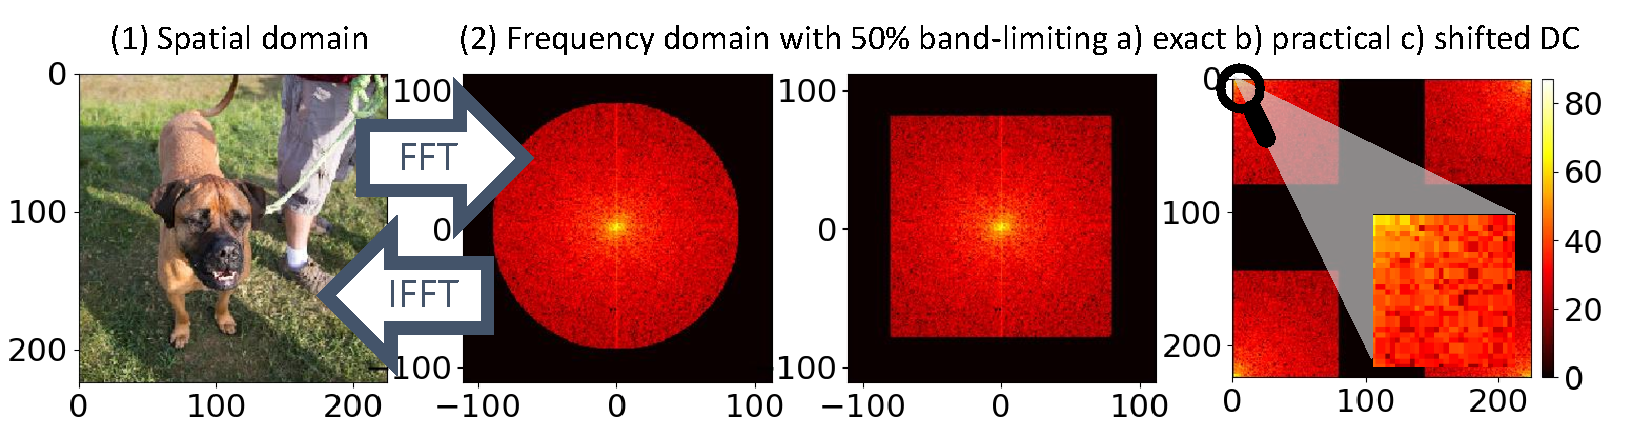
\includegraphics[width=\linewidth]{transformations_band_limiting_technique5.pdf} %width=\linewidth]
  \caption{{\it Transformations from input image to compressed FFT map. (1) Natural image in the spatial domain. (2) FFT transformation to frequency domain and a) exact band-limiting to 50\%, b) practical band-limiting to 50\%, c) lowest frequencies shifted to corners. The heat maps of magnitudes of Fourier coefficients are plotted for a single channel (0-th) in a logarithmic scale (dB) with linear interpolation and the max value is colored with white while the min value is colored with black.}}
  \label{fig:transforms}
\end{figure}

\begin{figure}[t]
  %
\includegraphics[width=\linewidth]{figures/conv2D-cifar10-leNet-test-accuracy.pdf} %width=\linewidth]
  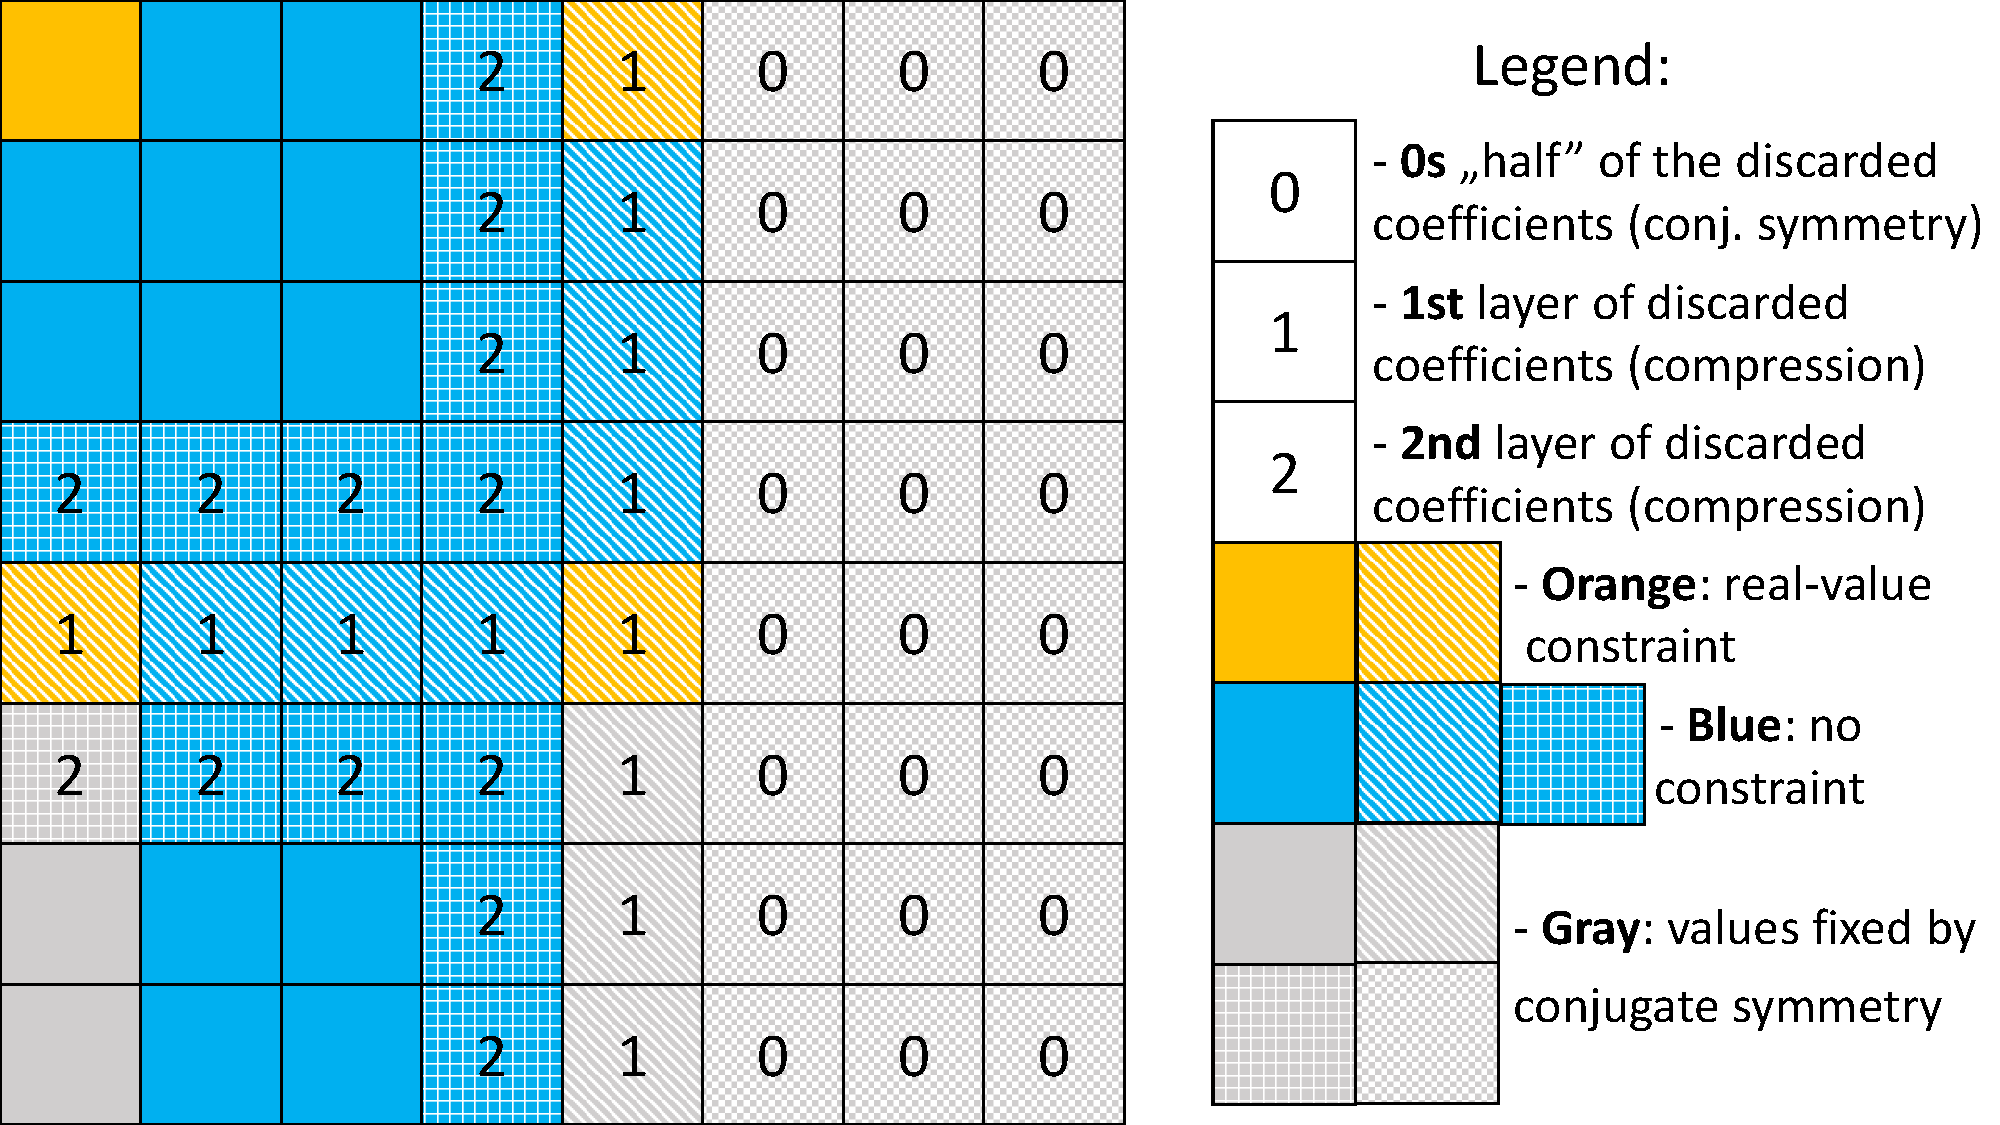
\includegraphics[width=\linewidth]{conjugateSymmetry.pdf} %width=\linewidth]
  \caption{{\it An example of a square input map with marked conjugate symmetry (\textbf{Gray} cells). 
  Almost \textit{half} of the input cells marked with \textbf{0}s (zeros) are discarded first due to the conjugate symmetry. The remaining map is compressed layer by layer (we present how the first two layers: \textbf{1} and \textbf{2} are selected). \textbf{Blue} and \textbf{Orange} cells represent a minimal number of coefficients that have to be preserved in the frequency domain to fully reconstruct the initial spatial input. Additionally, the \textbf{Orange} cells represent real-valued coefficients.}}
  \label{fig:conjugateSymmtry}
\end{figure}

The conjugate symmetry for a 2D signal $F[-\omega, -\theta] = F^*[\omega,\theta]$ is more complicated. If the real input map is of size $M \times N$, then its complex representation in the frequency domain is of size $M \times (\floor*{\frac{N}{2}} + 1)$. 
The real constraints for 2D inputs were explained in detail in Figure~\ref{fig:conjugateSymmtry}, similarly to~\cite{rippel2015spectral}. For the most interesting and most common case of even height and width of the input, there are always four real coefficients in the spectral representation (depicted as \textbf{Orange} cells: top-left corner, middle value in top row, middle value in most-left column and the value in the center). The DC component is located in the top-left corner. The largest values are placed in the corners and decrease
% in a \textit{"L" shaped (or quadrant)} fashion
% in a \textit{circular} fashion
towards the center. This trend is our guideline in the design of the compression pattern, in which for the \textit{left half} of the input, we discard coefficients from the center in \textit{L-like} shapes towards the top-left and bottom-left corners.

\subsubsection{Map Reuse}
\iffalse
\begin{figure}[t]
\centering
  %
\includegraphics[width=\linewidth]{figures/conv2D-cifar10-leNet-test-accuracy.pdf} %width=\linewidth]
  
\includegraphics[width=0.8\linewidth]{intuition.png} %width=\linewidth]
  \caption{{\it We visualize the effects of frequency-domain compression on the input layer (by compressing and decompressing an image). Even with a 50\% compression ratio the input is imperceptibly changed. Our approach generalizes this methodology to each of the layers of the convolutional neural network--compressing BOTH the inputs and the filters.}}
  \label{fig:intuiton}
\end{figure}
\fi

The FFT computations of the tensors: input map, filter, and the gradient of the output as well as the IFFT of the final output tensors are one of the most expensive operations in the FFT-based convolution. We avoid re-computation of the FFT for the input map and the filter by saving their frequency representations at the end of the forward pass and reusing them in the corresponding backward pass. The memory footprint for the input map in the spatial and frequency domains is almost the same. We retain only half of the frequency coefficients but they are represented as complex numbers. Further on, we assume square input maps and filters (the most common case). For an $N \times N$ real input map, the initial $\text{\textit{complex-size}}$ is $N \times (\floor*{\frac{N}{2}} + 1)$. The filter (also called kernel) is of size $K \times K$. The FFT-ed input map has to be convolved with the gradient of size $G \times G$ in the backward pass and usually $G > K$. Thus, to reuse the FFT-ed input map and avoid wrapped-around values, the required padding is of size: $P=\text{max}(K - 1, G - 1)$. This gives us the final full spatial size of tensors used in FFT operations $(N + P) \times (N + P)$ and the corresponding full \textit{complex-size} $(N + P) \times (\floor*{\frac{(N + P)}{2}} + 1)$ that is finally compressed.

\subsection{Implementation in PyTorch and CUDA}
Our compression in the frequency domain is implemented as a module in PyTorch that can be plugged into any architecture as a convolutional layer. The code is written in Python with extensions in C++ and CUDA for the main bottleneck of the algorithm. The most expensive computationally and memory-wise component is the Hadamard product in the frequency domain. The complexity analysis of the FFT-based convolution is described in~\cite{mathieu2013fast} (section 2.3, page 3). The complex multiplications for the convolution in the frequency domain require $3S·f'·f·n^2$ real multiplications and $5S·f'·f·n^2$ real additions, where $S$ is the mini-batch size, $f'$ is the number of filter banks (i.e., kernels or output channels), $f$ is the number of input channels, and $n$ is the height and width of the inputs. In comparison, the cost of the FFT of the input map is $S·f·n^2·2 log  n$, and usually $f' >> 2 log n$. We implemented in CUDA the fast algorithm to multiply complex numbers with 3 real multiplications instead of 4 as described in~\cite{Lavin2016FastConvolution}.

Our approach to convolution in the frequency domain aims at saving memory and utilizing as many GPU threads as possible. In our CUDA code, we fuse the element-wise complex multiplication (which in a standalone version is an injective one-to-one map operator) with the summation along an input channel (a reduction operator) in a thread execution path to limit the memory size from $2Sff'n^2$, where 2 represents the real and imaginary parts, to the size of the output $2Sf'n^2$, and avoid any additional synchronization by focusing on computation of a single output cell: $(x,y)$ coordinates in the output map. We also implemented another variant of convolution in the frequency domain by using tensor transpositions and replacing the complex tensor multiplication (CGEMM) with three real tensor multiplications (SGEMM).

\iffalse
\section{Application of Fast Fourier Transform to Convolution}
Our first goal is to implement convolutional layers using different methods and compare their performance.

\begin{figure}[t]
  \includegraphics[width=\linewidth]{compareFFT3.pdf} % width=\linewidth]
  \caption{{\it A comparison of convolution operations implemented in different frameworks and using various FFT versions for one-dimensional signals.}}                                        
  \label{fig:compareFFT}
\end{figure}

We implement a naive version of convolution (with many for loops - for each data point in the mini-batch, channel, and each dimension in the input) to serve as our baseline and the ground truth in terms of the returned value. Next, we implement convolution via FFT. The algorithm is written according to the schema presented in~\cite{numericalRecipes} (chapter 13). It is worth noting that the pre-processing steps are crucial for a correct implementation of convolution via FFT. The filter is usually much smaller (than the input) and has to be padded with zeros to the final length of the input signal. The input signal has to be padded on both ends with as many zeros as the size of the filter to prevent the effects of wrapped-around filter data (for example, the last values of convolution should be calculated only from the final overlap of the filter and input signal and should not be polluted with values from the beginning of the input signal).

Our first implementation of FFT-based convolution is in Python using \textit{numpy.fft} library. Subsequently, the convolution operation is used to implement the forward and backward pass of the convolutional layer (with focus on 1D case). We also test the performance of FFTW~\cite{fftw}. Interestingly enough, it is significantly slower (even about 10X) for 1D convolution than \textit{numpy.fft}. On the other hand, FFTW showed better performance than \textit{numpy.fft} for 2D convolution. We also examine cross-correlation (which is actually used in convolutional networks) from scipy. It has an interesting feature exposed for 1D case. We can choose 3 modes of execution: fft (computing cross-correlation via fft), direct (computation), auto (choose direct or fft method depending on which one is predicted to run faster). Thus, scipy provides a simplified optimizer to select the calculation of convolution (either via FFT or direct method) depending on cost estimation of each method. Internally, scipy calls fft from \textit{numpy.fft}. There is a crossover point between convolution via fft and direct one. For example, for a signal of input size 4096, the convolution via fft is faster for filters of size greater than about 300. For very small sizes of filter and input, the overhead of the auto mode (the optimization version in scipy) is large (probably scipy could be changed to always select the direct convolution for number of required multiplications below $2^{20}$).

\textbf{PyTorch} standard implementation of convolution is surprisingly slower than scipy or numpy and even there is a crossover point between our FFT-based convolution and the one from PyTorch. We also test GPU-based convolution from PyTorch and for input signal of size 4096, it is superior to all other implementations.

The fft based convolution from papers~\cite{lecunFFTLong, fbfftLong} is not incorporated into the standard version of PyTorch but have to be installed separately~\cite{fbcunn}.

\section{Compression in the frequency domain}

  \begin{figure}[t]
  \centering
  \includegraphics[width=\linewidth]{diagramFFTCompression.pdf} % width=\linewidth]
  \caption{{\it Compression applied to filters and activation input maps for FFT-based convolution with detailed annotation of steps to save memory and computation.}}
  \label{fig:diagramFFTCompression}        
  \end{figure}

\label{sec:compression}
Our focus is on how to compress a signal and filter in the frequency domain so that the relative error\footnote{Relative error definition:\\ ``https://en.wikipedia.org/wiki/Approximation\_error``} between the output of the convolution and the gold standard~\footnote{The standard version of convolution computed directly in the time domain.} is small. To be more precise, we want to compute convolution using FFT. The input to the convolution (e.g. a speech signal, time-series data, or an image) and a filter (also called kernel) are transformed from the time-domain to the frequency domain via FFT. Then we compress both the signal and the filter by discarding high frequency coefficients (the intuition is that we want to discard noise that is usually of high frequency). The number of discarded coefficients is chosen based on how much energy we want to preserve from the input signal (usually the filters are smaller than the input so easier to compress, thus we focus on the compression of the input signal). Finally, we apply the inverse FFT to go back to the time domain (see Figure: ~\ref{fig:diagramFFTCompression}).

We observe that the relative errors: $\delta = 100\% \frac{|V - V_{\mathrm{approx}}|}{|V| + |V_{\mathrm{approx}}|}$ (where $V$ is the input signal, $V_{\mathrm{approx}}$ is the approximation of the input signal after applying compression)  between gold standard and output of the convolution via FFT are relatively high (for example, after preserving 99.9\% energy of a signal, we discard about 100 coefficients out of 270 and get the relative errors of about 0.03). We check if similar errors are obtained when we compare the input signal with the same signal after its compression in the frequency domain. It occurs that this is the case, hence the compression in the frequency domain causes high numerical (relative) errors. However, the shape of the input signal and the output signal (after compression) are very similar visually (the errors can be discerned only when we zoom-in our graphs).

We considered using sparse FFT (SFFT~\cite{sparsefft}) but it shows better performance than FFTW~\cite{fftw} only for very long input signals. The results presented on the main page~\cite{sparsefft} indicate that SFFT outperforms FFTW for signals of size at least $2^{13}$, however, the maximum length of the signal that we currently are dealing with in one dimension is $2^{12}$. For this reason, we decided not to follow this path.

We tested an end-to-end performance of a simple 3 layer neural network with our FFT-based convolution. The main goal was to check if the relative errors introduced by the compression in the frequency domain have an impact on the training of a model. Our network has the following architecture: \textit{conv - relu - max pool - affine (fully connected) - relu - affine (fully connected) - softmax}. We used 32 one dimensional filters of size 49 each, a single data point is an array of 4096 values with 3 channels, the max pool is with pool width 2 and stride 2. This small network is sufficient to train a model for CIFAR-10 data (with 10 classes) and obtain accuracy above 90\%. To simulate 1 dimensional data, we reshaped each image from shape 3x64x64 to 3x4096 (the 3 channels were retained and the 64x64 image was translated to an array with 4096 values). The sanity check was for 10 training images. The loss was decreasing in the same way for uncompressed and compressed versions of convolution. Next, we tested our version of convolution on bigger data sizes. Our current code is not fully optimized so each epoch took about 20 min for 3000 test data points and 300 training data points. We ran 15 epochs for different variants of our convolutional layer. For example, when no compression was used (the output of the convolution had the relative error to the gold standard in the ballpark of about $10^{-14}$) the model achieved the train accuracy of about 70\% and the validation accuracy of about 45\%. When we used our compressed version of convolution, the model was able to achieve the training accuracy of about 55\% and the validation accuracy of about 40\% (with 98\% of the energy of the signal preserved). Moreover, the results for the compressed convolution were fluctuating and even with more energy preserved we were getting worse results. This indicates that the relative errors introduced by the compressed convolution propagate to the training of the models and demonstrate in the slower learning process.

Finally, we train the 3 layer network for many days to see if the loss of information inhibits the network from learning. In Figure~\ref{fig:500epochs}, we present results of many day training, where most models are able to reach 500 epochs. We observe that even the highly compressed signal with only 95\% of retained energy is able to achieve high accuracy values of about 90\%, however, it takes more epochs than for other models that do not apply compression. The most interesting result is that the pure calculation of convolution in the frequency domain without any compression is achieving 90\% accuracy faster than the models which compute convolution directly. It is worth noting that our convolution without any compression in the frequency domain has very small relative errors (from $10^{-10}$ to $10^{-12}$) in comparison to the results of direct convolution. Our conjecture why it happens is that the FFT based convolution exhibits some smoothing effect. When we go from the time domain to the frequency domain, the Fourier coefficient exhibit symmetry in the frequency domain. We take advantage of it and cut off half of the coefficients to save memory and number of multiplications. We checked if the two halves of the signal in the frequency domain are the same and it occurs that there are some small numerical differences of about $10^{-12}$. After computing convolution in the frequency domain, we restore the signal by mirroring it and taking its conjugate. This perfectly symmetrical output signal might be a better output than the result of direct convolution with small numerical errors.

The outcome of the non-compressed version of convolution suggests that the compression might have a detrimental effect, on both training time and number of epochs to reach a certain accuracy value. We obtain an interesting result. In Figure~\ref{fig:500epochs}, the models that use compression on both the input signal and the filter, with 95\% energy preserved or after removing a single Fourier coefficient, indeed, are learning slower than the models based on direct convolution (lines labeled: train\_acc naive and train\_acc numpy). On the other hand, the model with 99\% of compression applied is learning faster than the models based on the direct convolution. We think that this effect can be explained in two ways. First, the initialization of the models is random (even though we initialize the seed, the slight change in the environment or change in the filter size) does affect the learning process. In another experiment, where we use only a different pool width (5 instead of 3), model with 98\% compressed energy was learning faster than a model with 99\% compressed energy (at least for the first 15 epochs - the result is shown in Appendix). Another explanation is that we might not have handled all the corner cases in our version of compressed convolution. The method of spectral pooling (that we describe in Section~\ref{sec:spectralPooling}), suggests different handling of compression for the even and odd number of values in the output. We think that this slight inconsistency in the training results with compression might be because of lack of handling of the corner cases. We leave this issue as our future work.

The take-away from this analysis is that for the carefully chosen compression ratio we can learn as fast as standard models (with direct convolution) in terms of number of epochs, but faster in terms of total execution time (in this case for 99\% of preserved energy). 

\begin{figure}[t]   
  \centering                 
  \includegraphics[width=\linewidth]{500epochs2.pdf} % width=\linewidth]
  \caption{{\it Training accuracy with different types of convolutional layers applying various compression ratios (multi-day training).}}
  \label{fig:500epochs}
\end{figure}

  \subsection{Execution time and errors with compression for convolution} 
  
  \begin{figure}[t]       
  \centering        
  \includegraphics[width=\linewidth]{preservedEnergyExecutionTimeAbsError.png} % width=\linewidth]
  \caption{{\it Assessing how the preserved energy rate influences the execution time and the final absolute error of the convolution.}}                                  
  \label{fig:compareCompressionExecError}        
  \end{figure}

  Figure~\ref{fig:compareCompressionExecError} shows that a very high values of the preserved energy in the input signal corresponds to relatively small absolute error and a non-negligible speed-up of the convolution operation. The experiment confirms our expectation that the higher the compression ratio, the larger the error (between the direct result of convolution and the convolution computed in the frequency domain after compression of the input signal and filter). For very high compression ratios, the error surges and also the performance of the convolution plateaus. The 95\% of the preserved energy in the input is the lowest acceptable value for the 50words dataset from the UCR benchmark.

\section{Tests for speech data}
\begin{figure}[t]
  \centering           
  \includegraphics[width=\linewidth]{speechResults4.pdf} %width=\linewidth]
  \caption{{\it Training accuracy with different types of convolutional layers applying various compression ratios for the Switchboard dataset.}}
  \label{fig:speechResults}  
\end{figure}

We also train the same network as in Section~\ref{sec:compression} for the speech data from the Switchboard corpus of English conversational telephone speech. Data is parameterized as Mel-frequency cepstral coefficients with the first and second order derivatives. For the training set we use the set of about 4k word tokens. We leverage the code published for the paper~\cite{KamperLivescu2016} to process the data. We choose tokens that occur at least 14 times in the training set so that the size of the training set allows us to test convolutions with many different compression ratios. The input data is divided into batches of size 50, we treat each data point as a one-dimensional signal with 39 channels and 200 values in each channel.
%The corresponding dev and test sets are of sizes 2078 and 3509, respectively. Here we are primarily concerned with how much faster we can train (decrease the training accuracy) using the FFT for convolution.
Similarly to CIFAR-10 data we use 32 filters with size 49 each. Number of classes is 129. The training accuracy above 90\% is achieved after 45 epochs (99\% after 83 epochs) for the network where convolutions were computed using FFT and without any compression (we do not even smooth the signals via mirroring two halves in the frequency domain). We present the results in Figure~\ref{fig:speechResults}.

The results for Swtichboard data are better than the ones for CIFAR-10. We observe consistency, the lower level of preserved energy, the longer training. However, we can train as fast as a standard model with 90\% preserved energy. This result is probably because of more information per a single data point in the Switchboard dataset. It shows that we can efficiently compress the speech signals and learn much faster with compressed version of convolution in the frequency domain.

%It is worth mentioning that the code used for the experiments was written in Python using numpy to support all required operations for FFT. We made an effort to port it to PyTorch to use GPU, however, the PyTorch framework does not support complex numbers. A solution to it is to move to another framework, for example, we verified that TensorFlow does support complex numbers (and the automatic back-propagation for operations on complex numbers).
\fi